\documentclass{standalone}
\usepackage{tikz}
\usepackage{ctex,siunitx,ninecolors}
\setCJKmainfont{Noto Serif CJK SC}
\usepackage{tkz-euclide}
\usepackage{amsmath}
\usetikzlibrary{patterns, calc}
\usetikzlibrary {decorations.pathmorphing, decorations.pathreplacing, decorations.shapes,}
\begin{document}
\small
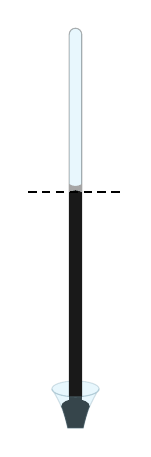
\begin{tikzpicture}[>=latex,scale=1.0]
  % \useasboundingbox(-1.4,-1.4)rectangle(1.4,1.4);
  \fill(0,-0.22)ellipse(0.18 and 0.09);
  \fill(0.18,-0.22)to[bend right=3](0.1,-0.5)--(-0.1,-0.5)to[bend right=3](-0.18,-0.22);
  \fill[black,draw=black](-0.08,-0.4)rectangle(0.08,-0.1);
  \fill[cyan!30!white,opacity=0.3,draw=cyan!30!gray,line join =round](-0.3,0)to[bend left=10](-0.1,-0.5)--(0.1,-0.5)to[bend left=10](0.3,0)arc(0:-180:0.3 and 0.1);
  \fill[cyan!30!white,opacity=0.3,draw=cyan!30!gray](0,0)ellipse(0.3 and 0.1);
  \fill[cyan!30!white,opacity=0.3,draw=black](-0.08,-0.1)--(-0.08,4.5)arc(180:0:0.08)--(0.08,-0.1);
  \fill[black!90](0.08,-0.1)--(0.08,2.5)to[bend right](-0.08,2.5)--(-0.08,-0.1)--cycle;
  \fill[gray!70](0.08,2.6)to[bend left](-0.08,2.6)--(-0.08,2.5)to[bend left](0.08,2.5)--cycle;
  \draw[densely dashed](-0.6,2.5)--(0.6,2.5);
\end{tikzpicture}
\end{document}